



    
% !TeX spellcheck = de_DE
% !TeX encoding = UTF-8
\documentclass{scrreprt}
\usepackage{ngerman}

    
    
    \usepackage[T1]{fontenc}
    % Nicer default font (+ math font) than Computer Modern for most use cases
    \usepackage{mathpazo}

    % Basic figure setup, for now with no caption control since it's done
    % automatically by Pandoc (which extracts ![](path) syntax from Markdown).
    \usepackage{graphicx}
    % We will generate all images so they have a width \maxwidth. This means
    % that they will get their normal width if they fit onto the page, but
    % are scaled down if they would overflow the margins.
    \makeatletter
    \def\maxwidth{\ifdim\Gin@nat@width>\linewidth\linewidth
    \else\Gin@nat@width\fi}
    \makeatother
    \let\Oldincludegraphics\includegraphics
    % Set max figure width to be 80% of text width, for now hardcoded.
    \renewcommand{\includegraphics}[1]{\Oldincludegraphics[width=.8\maxwidth]{#1}}
    % Ensure that by default, figures have no caption (until we provide a
    % proper Figure object with a Caption API and a way to capture that
    % in the conversion process - todo).
    \usepackage{caption}
    \DeclareCaptionLabelFormat{nolabel}{}
    \captionsetup{labelformat=nolabel}

    \usepackage{adjustbox} % Used to constrain images to a maximum size 
    \usepackage{xcolor} % Allow colors to be defined
    \usepackage{enumerate} % Needed for markdown enumerations to work
    \usepackage{geometry} % Used to adjust the document margins
    \usepackage{amsmath} % Equations
    \usepackage{amssymb} % Equations
    \usepackage{textcomp} % defines textquotesingle
    % Hack from http://tex.stackexchange.com/a/47451/13684:
    \AtBeginDocument{%
        \def\PYZsq{\textquotesingle}% Upright quotes in Pygmentized code
    }
    \usepackage{upquote} % Upright quotes for verbatim code
    \usepackage{eurosym} % defines \euro
    \usepackage[mathletters]{ucs} % Extended unicode (utf-8) support
    \usepackage[utf8x]{inputenc} % Allow utf-8 characters in the tex document
    \usepackage{fancyvrb} % verbatim replacement that allows latex
    \usepackage{grffile} % extends the file name processing of package graphics 
                         % to support a larger range 
    % The hyperref package gives us a pdf with properly built
    % internal navigation ('pdf bookmarks' for the table of contents,
    % internal cross-reference links, web links for URLs, etc.)
    \usepackage{hyperref}
    \usepackage{longtable} % longtable support required by pandoc >1.10
    \usepackage{booktabs}  % table support for pandoc > 1.12.2
    \usepackage[inline]{enumitem} % IRkernel/repr support (it uses the enumerate* environment)
    \usepackage[normalem]{ulem} % ulem is needed to support strikethroughs (\sout)
                                % normalem makes italics be italics, not underlines
    

    
    
    % Colors for the hyperref package
    \definecolor{urlcolor}{rgb}{0,.145,.698}
    \definecolor{linkcolor}{rgb}{.71,0.21,0.01}
    \definecolor{citecolor}{rgb}{.12,.54,.11}

    % ANSI colors
    \definecolor{ansi-black}{HTML}{3E424D}
    \definecolor{ansi-black-intense}{HTML}{282C36}
    \definecolor{ansi-red}{HTML}{E75C58}
    \definecolor{ansi-red-intense}{HTML}{B22B31}
    \definecolor{ansi-green}{HTML}{00A250}
    \definecolor{ansi-green-intense}{HTML}{007427}
    \definecolor{ansi-yellow}{HTML}{DDB62B}
    \definecolor{ansi-yellow-intense}{HTML}{B27D12}
    \definecolor{ansi-blue}{HTML}{208FFB}
    \definecolor{ansi-blue-intense}{HTML}{0065CA}
    \definecolor{ansi-magenta}{HTML}{D160C4}
    \definecolor{ansi-magenta-intense}{HTML}{A03196}
    \definecolor{ansi-cyan}{HTML}{60C6C8}
    \definecolor{ansi-cyan-intense}{HTML}{258F8F}
    \definecolor{ansi-white}{HTML}{C5C1B4}
    \definecolor{ansi-white-intense}{HTML}{A1A6B2}

    % commands and environments needed by pandoc snippets
    % extracted from the output of `pandoc -s`
    \providecommand{\tightlist}{%
      \setlength{\itemsep}{0pt}\setlength{\parskip}{0pt}}
    \DefineVerbatimEnvironment{Highlighting}{Verbatim}{commandchars=\\\{\}}
    % Add ',fontsize=\small' for more characters per line
    \newenvironment{Shaded}{}{}
    \newcommand{\KeywordTok}[1]{\textcolor[rgb]{0.00,0.44,0.13}{\textbf{{#1}}}}
    \newcommand{\DataTypeTok}[1]{\textcolor[rgb]{0.56,0.13,0.00}{{#1}}}
    \newcommand{\DecValTok}[1]{\textcolor[rgb]{0.25,0.63,0.44}{{#1}}}
    \newcommand{\BaseNTok}[1]{\textcolor[rgb]{0.25,0.63,0.44}{{#1}}}
    \newcommand{\FloatTok}[1]{\textcolor[rgb]{0.25,0.63,0.44}{{#1}}}
    \newcommand{\CharTok}[1]{\textcolor[rgb]{0.25,0.44,0.63}{{#1}}}
    \newcommand{\StringTok}[1]{\textcolor[rgb]{0.25,0.44,0.63}{{#1}}}
    \newcommand{\CommentTok}[1]{\textcolor[rgb]{0.38,0.63,0.69}{\textit{{#1}}}}
    \newcommand{\OtherTok}[1]{\textcolor[rgb]{0.00,0.44,0.13}{{#1}}}
    \newcommand{\AlertTok}[1]{\textcolor[rgb]{1.00,0.00,0.00}{\textbf{{#1}}}}
    \newcommand{\FunctionTok}[1]{\textcolor[rgb]{0.02,0.16,0.49}{{#1}}}
    \newcommand{\RegionMarkerTok}[1]{{#1}}
    \newcommand{\ErrorTok}[1]{\textcolor[rgb]{1.00,0.00,0.00}{\textbf{{#1}}}}
    \newcommand{\NormalTok}[1]{{#1}}
    
    % Additional commands for more recent versions of Pandoc
    \newcommand{\ConstantTok}[1]{\textcolor[rgb]{0.53,0.00,0.00}{{#1}}}
    \newcommand{\SpecialCharTok}[1]{\textcolor[rgb]{0.25,0.44,0.63}{{#1}}}
    \newcommand{\VerbatimStringTok}[1]{\textcolor[rgb]{0.25,0.44,0.63}{{#1}}}
    \newcommand{\SpecialStringTok}[1]{\textcolor[rgb]{0.73,0.40,0.53}{{#1}}}
    \newcommand{\ImportTok}[1]{{#1}}
    \newcommand{\DocumentationTok}[1]{\textcolor[rgb]{0.73,0.13,0.13}{\textit{{#1}}}}
    \newcommand{\AnnotationTok}[1]{\textcolor[rgb]{0.38,0.63,0.69}{\textbf{\textit{{#1}}}}}
    \newcommand{\CommentVarTok}[1]{\textcolor[rgb]{0.38,0.63,0.69}{\textbf{\textit{{#1}}}}}
    \newcommand{\VariableTok}[1]{\textcolor[rgb]{0.10,0.09,0.49}{{#1}}}
    \newcommand{\ControlFlowTok}[1]{\textcolor[rgb]{0.00,0.44,0.13}{\textbf{{#1}}}}
    \newcommand{\OperatorTok}[1]{\textcolor[rgb]{0.40,0.40,0.40}{{#1}}}
    \newcommand{\BuiltInTok}[1]{{#1}}
    \newcommand{\ExtensionTok}[1]{{#1}}
    \newcommand{\PreprocessorTok}[1]{\textcolor[rgb]{0.74,0.48,0.00}{{#1}}}
    \newcommand{\AttributeTok}[1]{\textcolor[rgb]{0.49,0.56,0.16}{{#1}}}
    \newcommand{\InformationTok}[1]{\textcolor[rgb]{0.38,0.63,0.69}{\textbf{\textit{{#1}}}}}
    \newcommand{\WarningTok}[1]{\textcolor[rgb]{0.38,0.63,0.69}{\textbf{\textit{{#1}}}}}
    
    
    % Define a nice break command that doesn't care if a line doesn't already
    % exist.
    \def\br{\hspace*{\fill} \\* }
    % Math Jax compatability definitions
    \def\gt{>}
    \def\lt{<}
    % Document parameters
    \title{Capstone Proposal}
    
    
    

    % Pygments definitions
    
\makeatletter
\def\PY@reset{\let\PY@it=\relax \let\PY@bf=\relax%
    \let\PY@ul=\relax \let\PY@tc=\relax%
    \let\PY@bc=\relax \let\PY@ff=\relax}
\def\PY@tok#1{\csname PY@tok@#1\endcsname}
\def\PY@toks#1+{\ifx\relax#1\empty\else%
    \PY@tok{#1}\expandafter\PY@toks\fi}
\def\PY@do#1{\PY@bc{\PY@tc{\PY@ul{%
    \PY@it{\PY@bf{\PY@ff{#1}}}}}}}
\def\PY#1#2{\PY@reset\PY@toks#1+\relax+\PY@do{#2}}

\expandafter\def\csname PY@tok@sr\endcsname{\def\PY@tc##1{\textcolor[rgb]{0.73,0.40,0.53}{##1}}}
\expandafter\def\csname PY@tok@gs\endcsname{\let\PY@bf=\textbf}
\expandafter\def\csname PY@tok@go\endcsname{\def\PY@tc##1{\textcolor[rgb]{0.53,0.53,0.53}{##1}}}
\expandafter\def\csname PY@tok@s2\endcsname{\def\PY@tc##1{\textcolor[rgb]{0.73,0.13,0.13}{##1}}}
\expandafter\def\csname PY@tok@kt\endcsname{\def\PY@tc##1{\textcolor[rgb]{0.69,0.00,0.25}{##1}}}
\expandafter\def\csname PY@tok@sb\endcsname{\def\PY@tc##1{\textcolor[rgb]{0.73,0.13,0.13}{##1}}}
\expandafter\def\csname PY@tok@il\endcsname{\def\PY@tc##1{\textcolor[rgb]{0.40,0.40,0.40}{##1}}}
\expandafter\def\csname PY@tok@o\endcsname{\def\PY@tc##1{\textcolor[rgb]{0.40,0.40,0.40}{##1}}}
\expandafter\def\csname PY@tok@mh\endcsname{\def\PY@tc##1{\textcolor[rgb]{0.40,0.40,0.40}{##1}}}
\expandafter\def\csname PY@tok@cs\endcsname{\let\PY@it=\textit\def\PY@tc##1{\textcolor[rgb]{0.25,0.50,0.50}{##1}}}
\expandafter\def\csname PY@tok@nv\endcsname{\def\PY@tc##1{\textcolor[rgb]{0.10,0.09,0.49}{##1}}}
\expandafter\def\csname PY@tok@mf\endcsname{\def\PY@tc##1{\textcolor[rgb]{0.40,0.40,0.40}{##1}}}
\expandafter\def\csname PY@tok@ch\endcsname{\let\PY@it=\textit\def\PY@tc##1{\textcolor[rgb]{0.25,0.50,0.50}{##1}}}
\expandafter\def\csname PY@tok@nn\endcsname{\let\PY@bf=\textbf\def\PY@tc##1{\textcolor[rgb]{0.00,0.00,1.00}{##1}}}
\expandafter\def\csname PY@tok@gt\endcsname{\def\PY@tc##1{\textcolor[rgb]{0.00,0.27,0.87}{##1}}}
\expandafter\def\csname PY@tok@kr\endcsname{\let\PY@bf=\textbf\def\PY@tc##1{\textcolor[rgb]{0.00,0.50,0.00}{##1}}}
\expandafter\def\csname PY@tok@sc\endcsname{\def\PY@tc##1{\textcolor[rgb]{0.73,0.13,0.13}{##1}}}
\expandafter\def\csname PY@tok@sh\endcsname{\def\PY@tc##1{\textcolor[rgb]{0.73,0.13,0.13}{##1}}}
\expandafter\def\csname PY@tok@gi\endcsname{\def\PY@tc##1{\textcolor[rgb]{0.00,0.63,0.00}{##1}}}
\expandafter\def\csname PY@tok@mo\endcsname{\def\PY@tc##1{\textcolor[rgb]{0.40,0.40,0.40}{##1}}}
\expandafter\def\csname PY@tok@nt\endcsname{\let\PY@bf=\textbf\def\PY@tc##1{\textcolor[rgb]{0.00,0.50,0.00}{##1}}}
\expandafter\def\csname PY@tok@nd\endcsname{\def\PY@tc##1{\textcolor[rgb]{0.67,0.13,1.00}{##1}}}
\expandafter\def\csname PY@tok@mi\endcsname{\def\PY@tc##1{\textcolor[rgb]{0.40,0.40,0.40}{##1}}}
\expandafter\def\csname PY@tok@kc\endcsname{\let\PY@bf=\textbf\def\PY@tc##1{\textcolor[rgb]{0.00,0.50,0.00}{##1}}}
\expandafter\def\csname PY@tok@nb\endcsname{\def\PY@tc##1{\textcolor[rgb]{0.00,0.50,0.00}{##1}}}
\expandafter\def\csname PY@tok@cpf\endcsname{\let\PY@it=\textit\def\PY@tc##1{\textcolor[rgb]{0.25,0.50,0.50}{##1}}}
\expandafter\def\csname PY@tok@vi\endcsname{\def\PY@tc##1{\textcolor[rgb]{0.10,0.09,0.49}{##1}}}
\expandafter\def\csname PY@tok@no\endcsname{\def\PY@tc##1{\textcolor[rgb]{0.53,0.00,0.00}{##1}}}
\expandafter\def\csname PY@tok@gd\endcsname{\def\PY@tc##1{\textcolor[rgb]{0.63,0.00,0.00}{##1}}}
\expandafter\def\csname PY@tok@bp\endcsname{\def\PY@tc##1{\textcolor[rgb]{0.00,0.50,0.00}{##1}}}
\expandafter\def\csname PY@tok@ge\endcsname{\let\PY@it=\textit}
\expandafter\def\csname PY@tok@nc\endcsname{\let\PY@bf=\textbf\def\PY@tc##1{\textcolor[rgb]{0.00,0.00,1.00}{##1}}}
\expandafter\def\csname PY@tok@si\endcsname{\let\PY@bf=\textbf\def\PY@tc##1{\textcolor[rgb]{0.73,0.40,0.53}{##1}}}
\expandafter\def\csname PY@tok@kd\endcsname{\let\PY@bf=\textbf\def\PY@tc##1{\textcolor[rgb]{0.00,0.50,0.00}{##1}}}
\expandafter\def\csname PY@tok@gu\endcsname{\let\PY@bf=\textbf\def\PY@tc##1{\textcolor[rgb]{0.50,0.00,0.50}{##1}}}
\expandafter\def\csname PY@tok@se\endcsname{\let\PY@bf=\textbf\def\PY@tc##1{\textcolor[rgb]{0.73,0.40,0.13}{##1}}}
\expandafter\def\csname PY@tok@err\endcsname{\def\PY@bc##1{\setlength{\fboxsep}{0pt}\fcolorbox[rgb]{1.00,0.00,0.00}{1,1,1}{\strut ##1}}}
\expandafter\def\csname PY@tok@s1\endcsname{\def\PY@tc##1{\textcolor[rgb]{0.73,0.13,0.13}{##1}}}
\expandafter\def\csname PY@tok@ne\endcsname{\let\PY@bf=\textbf\def\PY@tc##1{\textcolor[rgb]{0.82,0.25,0.23}{##1}}}
\expandafter\def\csname PY@tok@mb\endcsname{\def\PY@tc##1{\textcolor[rgb]{0.40,0.40,0.40}{##1}}}
\expandafter\def\csname PY@tok@kn\endcsname{\let\PY@bf=\textbf\def\PY@tc##1{\textcolor[rgb]{0.00,0.50,0.00}{##1}}}
\expandafter\def\csname PY@tok@cp\endcsname{\def\PY@tc##1{\textcolor[rgb]{0.74,0.48,0.00}{##1}}}
\expandafter\def\csname PY@tok@m\endcsname{\def\PY@tc##1{\textcolor[rgb]{0.40,0.40,0.40}{##1}}}
\expandafter\def\csname PY@tok@c1\endcsname{\let\PY@it=\textit\def\PY@tc##1{\textcolor[rgb]{0.25,0.50,0.50}{##1}}}
\expandafter\def\csname PY@tok@gr\endcsname{\def\PY@tc##1{\textcolor[rgb]{1.00,0.00,0.00}{##1}}}
\expandafter\def\csname PY@tok@c\endcsname{\let\PY@it=\textit\def\PY@tc##1{\textcolor[rgb]{0.25,0.50,0.50}{##1}}}
\expandafter\def\csname PY@tok@k\endcsname{\let\PY@bf=\textbf\def\PY@tc##1{\textcolor[rgb]{0.00,0.50,0.00}{##1}}}
\expandafter\def\csname PY@tok@ni\endcsname{\let\PY@bf=\textbf\def\PY@tc##1{\textcolor[rgb]{0.60,0.60,0.60}{##1}}}
\expandafter\def\csname PY@tok@vc\endcsname{\def\PY@tc##1{\textcolor[rgb]{0.10,0.09,0.49}{##1}}}
\expandafter\def\csname PY@tok@gp\endcsname{\let\PY@bf=\textbf\def\PY@tc##1{\textcolor[rgb]{0.00,0.00,0.50}{##1}}}
\expandafter\def\csname PY@tok@kp\endcsname{\def\PY@tc##1{\textcolor[rgb]{0.00,0.50,0.00}{##1}}}
\expandafter\def\csname PY@tok@vg\endcsname{\def\PY@tc##1{\textcolor[rgb]{0.10,0.09,0.49}{##1}}}
\expandafter\def\csname PY@tok@sx\endcsname{\def\PY@tc##1{\textcolor[rgb]{0.00,0.50,0.00}{##1}}}
\expandafter\def\csname PY@tok@cm\endcsname{\let\PY@it=\textit\def\PY@tc##1{\textcolor[rgb]{0.25,0.50,0.50}{##1}}}
\expandafter\def\csname PY@tok@ss\endcsname{\def\PY@tc##1{\textcolor[rgb]{0.10,0.09,0.49}{##1}}}
\expandafter\def\csname PY@tok@na\endcsname{\def\PY@tc##1{\textcolor[rgb]{0.49,0.56,0.16}{##1}}}
\expandafter\def\csname PY@tok@w\endcsname{\def\PY@tc##1{\textcolor[rgb]{0.73,0.73,0.73}{##1}}}
\expandafter\def\csname PY@tok@nl\endcsname{\def\PY@tc##1{\textcolor[rgb]{0.63,0.63,0.00}{##1}}}
\expandafter\def\csname PY@tok@s\endcsname{\def\PY@tc##1{\textcolor[rgb]{0.73,0.13,0.13}{##1}}}
\expandafter\def\csname PY@tok@ow\endcsname{\let\PY@bf=\textbf\def\PY@tc##1{\textcolor[rgb]{0.67,0.13,1.00}{##1}}}
\expandafter\def\csname PY@tok@sd\endcsname{\let\PY@it=\textit\def\PY@tc##1{\textcolor[rgb]{0.73,0.13,0.13}{##1}}}
\expandafter\def\csname PY@tok@nf\endcsname{\def\PY@tc##1{\textcolor[rgb]{0.00,0.00,1.00}{##1}}}
\expandafter\def\csname PY@tok@gh\endcsname{\let\PY@bf=\textbf\def\PY@tc##1{\textcolor[rgb]{0.00,0.00,0.50}{##1}}}

\def\PYZbs{\char`\\}
\def\PYZus{\char`\_}
\def\PYZob{\char`\{}
\def\PYZcb{\char`\}}
\def\PYZca{\char`\^}
\def\PYZam{\char`\&}
\def\PYZlt{\char`\<}
\def\PYZgt{\char`\>}
\def\PYZsh{\char`\#}
\def\PYZpc{\char`\%}
\def\PYZdl{\char`\$}
\def\PYZhy{\char`\-}
\def\PYZsq{\char`\'}
\def\PYZdq{\char`\"}
\def\PYZti{\char`\~}
% for compatibility with earlier versions
\def\PYZat{@}
\def\PYZlb{[}
\def\PYZrb{]}
\makeatother


    % Exact colors from NB
    \definecolor{incolor}{rgb}{0.0, 0.0, 0.5}
    \definecolor{outcolor}{rgb}{0.545, 0.0, 0.0}

    % Don't number sections
    \renewcommand{\thesection}{\hspace*{-0.5em}}
    \renewcommand{\thesubsection}{\hspace*{-0.5em}}



    
    % Prevent overflowing lines due to hard-to-break entities
    \sloppy 
    % Setup hyperref package
    \hypersetup{
      breaklinks=true,  % so long urls are correctly broken across lines
      colorlinks=true,
      urlcolor=urlcolor,
      linkcolor=linkcolor,
      citecolor=citecolor,
      }
    % Slightly bigger margins than the latex defaults
    
    \geometry{verbose,tmargin=1in,bmargin=1in,lmargin=1in,rmargin=1in}
    
    

    \begin{document}
    
    
    
    
    

    
    

    Trenton Potgieter

January 12, 2017

\section{A Three-Way Consensus Pipeline for Stress Level
Detection}\label{a-three-way-consensus-pipeline-for-stress-level-detection}

\subsection{1. Background}\label{background}

As one gets older, an increasingly difficult awareness of our parent's
mortality becomes a serious concern. Personally, my parents are both in
their early 70's and according to a study {[}\^{}1{]} done in
\textbf{2015} by the \textbf{American Heart Association}, around
\textbf{370,000} people die of heart attacks each year and is the
\textbf{No. 1} cause of in the United States. In \textbf{2014}, around
\textbf{356,500} people experienced heart attacks out of the hospital.
Of that amount only \textbf{12\%} survived due to emergency medical
services intervention. Personally, I would not like my parents to be one
the \textbf{88\%} who suffered from a fatal heart attack and didn't
survive due to the fact that there was no intervention by emergency
medical services. According to the study, there is a prevalence of
almost \emph{third} of the population at risk of \emph{Heart Disease}
leading to a \emph{Heart Attack} as one approaches \textbf{80+} years of
age. Having no personal experience in the Coronary Field of Medical
research, it would be difficult for me to diagnose any potential warning
signs, but with the advent of wearable technology, the mechanisms are in
place to potentially aid in this early warning and detection of heart
attacks. The majority of wearable technology today has the built-in
ability to monitor heart rates. Therefore in this project, I proposed
that this information can be uploaded or sent to a \textbf{data
ingestion pipeline} that this capable of interpreting, analyzing and
detecting an the patterns that could be classified as symptoms of a
heart attack.

Additionally, since one of the potential symptoms is the increase in
heart rates. There are a number of potential factors that influence the
increase in heart rate, but there are well published guidelines
{[}\^{}2{]} that can be used to determine anomalous patterns. If these
anomalies occur, the the \textbf{data ingestion pipeline} could
proactively determine if a heart attack is about to \emph{or} has
occurred and alert the appropriate emergency medical response. Thus
proactively preventing a fatal or near-fatal heart attack. As am added
benefit, the \textbf{pipeline} mechanism can be used to monitor patients
who are in \emph{Cardiac Rehabilitation} {[}\^{}3{]}.

\subsection{2. Problem Statement}\label{problem-statement}

For this Project, I propose creating a classification pipeline that
ingests heart-rate signal data (from a simulated wearable monitor) and
classifies whether the subject is in a stressful situation that could
lead to \emph{Cardiac Unrest}. Additionally, in order to prevent a
"cry-wolf" scenario or \emph{false-positives}, the pipeline employs a
consensus mechanism where three classifiers must all agree on the
classification.

\subsection{3. Datasets and Inputs}\label{datasets-and-inputs}

The dataset used for this Project was obtained as part of a \emph{Proof
of Concept (POC)} project in the \textbf{Dell IoT Solutions Lab}
{[}\^{}6{]} in Santa Clara, California, where a PPG {[}\^{}4{]} Pulse
sensor was used to measure Heart Rate Variability (HRV) {[}\^{}7{]}
reading, similar to those found on current wearables like the
\textbf{Fitbit Charge 2} {[}\^{}8{]}. The scope of the original POC is
simply to verify if the data can be extracted and filtered to detect
peaks in the PPG signal for a one minute data segment. Four separate
test subjects (between the ages of 68 and 76) were subjected to
different stimuli to induce \emph{stress} and \emph{relaxing} scenarios.
The one minute observations (\textbf{300} in total) are stored in a
\texttt{data.csv} file. Each observation has \textbf{8} specific
features of the PPG waveform, namely:

\begin{enumerate}
\def\labelenumi{\arabic{enumi}.}
\itemsep1pt\parskip0pt\parsep0pt
\item
  Time $\rightarrow$ Time Stamp of the observation.
\item
  AVRR $\rightarrow$ Average "normal" hert beats.
\item
  AVHR $\rightarrow$ Average total heart beats.
\item
  SDRR $\rightarrow$ Standard Deviation of "normal" heart beats.
\item
  RMSRR $\rightarrow$ Root Mean Squared of "normal" hear beats.
\item
  ppNN50 $\rightarrow$ Proportion of NN50 (50 successive "normal" heart
  beats) divided by total number of "normal" heart beats.
\item
  ppNN20 $\rightarrow$ Proportion of NN20 (20 successive "normal" heart
  beats) divided by total number of "normal" heart beats.
\item
  Label $\rightarrow$ Stressed or Relaxed.
\end{enumerate}

A sample of the data set is as follows:

    

    

    
    
    \begin{verbatim}
                Time       AVHR       AVRR      SDRR     RMSSD     ppNN50  \
0  07:16:37 25-08-15  74.393829  25.203703  1.883951  1.710125  16.666666   

      ppNN20  State  
0  22.222221  relax  
    \end{verbatim}

    

    To address the scope of this project however, I propose training three
separate supervised machine learning models by applying the following
methodology to create a pipeline:

\begin{enumerate}
\def\labelenumi{\arabic{enumi}.}
\itemsep1pt\parskip0pt\parsep0pt
\item
  Separate the input data into two separate repositories. One for the
  observations and one for the labeled output.
\item
  Apply \textbf{normalization} and/or \textbf{standardization}
  techniques to pre-process the data.
\item
  Define three separate models to evaluate the the data.
\end{enumerate}

\begin{quote}
\textbf{Note:} There are two concerns with the above dataset. The
\emph{first} is that fact that it has only 300 observations, thus making
it a relatively small data set. The \emph{second} is the fact that there
are significantly more observations labeled as \texttt{relaxed} then
there are those labeled as \texttt{stressed}. To address this
\emph{imbalance} and verify the accuracy of the predictions, I propose
leveraging \textbf{k-fold cross validation} to split the the data into a
\textbf{60\%} training set and a \textbf{30\%} testing set. This process
will be executed \textbf{10} times (10 Folds). The advantage of this
technique is that it can treat each test set uniquely, thus addressing
the fact that the data set used is relatively small, and provide an
average prediction result across the 10 folds. This process will be used
for each of the three models.
\end{quote}

\begin{enumerate}
\def\labelenumi{\arabic{enumi}.}
\setcounter{enumi}{3}
\itemsep1pt\parskip0pt\parsep0pt
\item
  Apply the models and measure their performance on a completely
  \textbf{separate} and as yet \textbf{unseen} dataset. This dataset is
  exactly the same as the training dataset except it is has no
  \texttt{State} label.
\end{enumerate}

\subsection{4. Solution}\label{solution}

Once created, the pipeline (see Section 7) will be used to test and
deploy the models on a sample unseen data from the test subjects and
hence predict their stress levels.

To accomplish this, the pipeline is comprised of three stages:

\begin{enumerate}
\def\labelenumi{\arabic{enumi}.}
\itemsep1pt\parskip0pt\parsep0pt
\item
  \textbf{Ingesting signal data}. $\rightarrow$ Collect already filtered
  PPG {[}\^{}4{]} signal data with symbolic peaks (and other features)
  have been collected for a one-minute time segment. Each one-minute
  time segment is considered an observation labeled with the class
  \texttt{relax} or \texttt{stress}.
\item
  \textbf{Classification model training}.
\item
  \textbf{Classification model application on new, unseen data}.
  $\rightarrow$ The final classification is Implementing a Weighted
  Majority Rule Ensemble Classifier {[}\^{}5{]} based on the probability
  of the time segment observation belonging to either class, using the
  following: \[
  \hat{y} = \arg\max_{i}\sum^{m}_{j=1}w_{j}p_{ij},
  \] where $wj$ is the weight that can be assigned to the $j^{th}$
  classifier.
\end{enumerate}

It is the objective of this project to re-apply the resulting pipeline
to a set of new test subjects and hopefully provide a viable prototype
that can preemptively warn of potential heart attacks. Based on this
final classification, additional future actions can be implemented that
are currently outside the scope of this project.

\subsection{5. Benchmark Model}\label{benchmark-model}

Since there isn't another comparable methodology for the proposed
pipeline and hence there isn't a comparable model implementation to
serve as a benchmark, the pipeline methodology will be compared to a
simple \textbf{Linear Classifier}. The evaluation criteria (see section
6) will be leveraged to compare each individual model's performance as
well as the final ensemble model's performance against the \emph{Linear
Classifier's} baseline.

\subsection{6. Evaluation Metrics}\label{evaluation-metrics}

Since the success criteria of the project is based on the overall
\textbf{probability} of the time segment observation belonging to either
class (\texttt{stressed} or \texttt{relaxed}), each individual model as
well as the overall consensus pipeline will be evaluated using the
following metrics:

\begin{enumerate}
\def\labelenumi{\arabic{enumi}.}
\item
  \textbf{Confusion Matrix:} $\rightarrow$ A tabular breakdown of
  predictions into a table showing the predictions that are correctly
  classified as well and the predictions are made incorrectly.
\item
  \textbf{Recall:} $\rightarrow$ The measure of completeness of the
  classifier. In other words, if the label is \texttt{stressed}, how
  well does the model predict that the subject is \texttt{stressed}.
  Basically, the ratio of the number of observations the model can
  correctly recall, to the number of all correct observations. \[
  Recall = \frac{True Positive}{True Positive + False Negative}
  \]
\item
  \textbf{Precision:} $\rightarrow$ The number of positive predictions
  divided by the total positive class values. So, precision is the ratio
  of a number of observations the model can correctly predict to a
  number of all observations the model can recall. In other words, it is
  how precise the model's recall is. \[
  Precision = \frac{True Positive}{True Positive + False Positive}
  \]
\item
  \textbf{F1 Score:} $\rightarrow$ If the models are good at
  \emph{Recall}, that doesn't necessarily mean that they are good at
  \emph{Precision}. The \emph{F1 Score} is the balanced average of the
  the two. This balanced \emph{F1 Score} is necessary as an overal
  performance metric due to the fact that if there is a
  misclassification that the subject is under stress, but isn't, then
  the emergency medical services are called out unnecessarily. If
  however, there is a misclassification that the subject isn't stressed,
  but actually is, then this could result in a fatality. Having the
  \emph{F1 Score} will allow us to allocate more weight to
  \emph{Precision} or \emph{Recall}. \[
  F1 \ Score = \frac{2 \cdot Precision}{Precision + Recall}
  \]
\end{enumerate}

\subsection{7. Overall Design}\label{overall-design}

\begin{figure}[htbp]
\centering
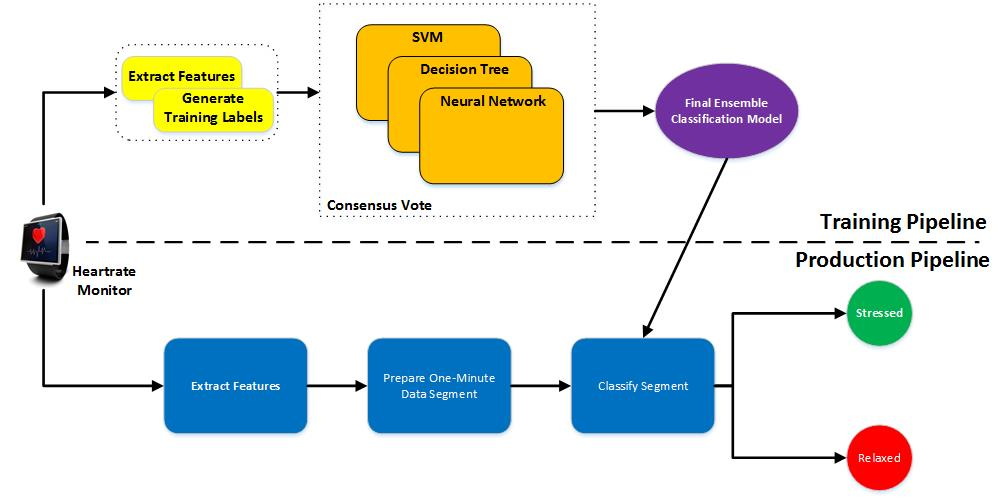
\includegraphics{images/Pipeline.jpg}
\caption{Figure 1: Training/Testing Pipeline}
\end{figure}

Figure 1 provides an overview of the proposed pipeline that address the
solution scope and is separated into two specific workflows:

\begin{enumerate}
\def\labelenumi{\arabic{enumi}.}
\itemsep1pt\parskip0pt\parsep0pt
\item
  Training
\item
  Production
\end{enumerate}

\subsubsection{7.1 The Training Pipeline}\label{the-training-pipeline}

The Training Pipeline is comprised of \emph{three} specific stages.

\paragraph{7.1.1 Feature Extraction}\label{feature-extraction}

The first process - \textbf{Feature Extraction} - separates the incoming
signal data from the heart rate monitor into two separate training data
sets. The first data set are the signal observations, while the second
data set are the training labels associated with each observation. The
labels are further converted to a binary integer value, demarcating $1$
for \texttt{relaxed} and $0$ for \texttt{stressed}. Additionally, in
order to account for outlier variables and overfitting, the data is
further standardized and scaled using the following:

\begin{quote}
\textbf{Standardize:} \[
X = \frac{\sum^{n}_{i=1}(x_{i} - \mu)}{\sigma}
\]
\end{quote}

\begin{quote}
\textbf{Scale:} \[
X' = \frac{X - X_{min}}{X_{max} - X_{min}}
\]
\end{quote}

\paragraph{7.1.2 Model Training}\label{model-training}

Once the data has been pre-processed, three separate classifieds are
trained on the data.

\begin{enumerate}
\def\labelenumi{\arabic{enumi}.}
\itemsep1pt\parskip0pt\parsep0pt
\item
  Decision Tree
\item
  Support Vector Machines (SVM)
\item
  Neural Network
\end{enumerate}

Once each of these models have been trained, there resultant
classification probability undergoes a consensus vote to determine the
the final classification probability by by using the \textbf{Weighted
Average Probabilities} ensemble method.

\paragraph{7.1.3 Final Model}\label{final-model}

The last stage of the Training Pipeline is an optimized classification
model that can be used for new data.

\subsubsection{7.2 Testing/Production
Pipeline}\label{testingproduction-pipeline}

Like the Training Pipeline, the Production/Testing Pipeline also
comprises of three stages.

\paragraph{7.2.1 Feature Extraction}\label{feature-extraction-1}

Unlike the first stage of the Training Pipeline, the data from the heart
rate monitor is not separated into two data sets. Rather, the signal
data is pre-processed; scaled and normalized.

\paragraph{7.2.2 Observation
Segmentation}\label{observation-segmentation}

The pre-processed data is then split into one-minute segments based on
the time stamp of the data. These one-minute segments are established as
a single observation of the test individuals stress level at the given
time.

\paragraph{7.2.3 Classification}\label{classification}

The final model from the Training Pipeline is then executed against each
one-minute observation segment to classify whether the test subject is
\texttt{stressed} or \texttt{relaxed}.

\subsection{8. References}\label{references}

\begin{enumerate}
\def\labelenumi{\arabic{enumi}.}
\itemsep1pt\parskip0pt\parsep0pt
\item
  https://www.heart.org/idc/groups/ahamah-public/@wcm/@sop/@smd/documents/downloadable/ucm\_480086.pdf
\item
  http://www.heart.org/HEARTORG/HealthyLiving/PhysicalActivity/FitnessBasics/Target-Heart-Rates\_UCM\_434341\_Article.jsp\#.WHEiXbGZNE4)
\item
  https://www.nhlbi.nih.gov/health/health-topics/topics/rehab
\item
  https://en.wikipedia.org/wiki/Photoplethysmogram
\item
  http://scikit-learn.org/stable/modules/ensemble.html\#weighted-average-probabilities-soft-voting
\item
  https://www.dell.com/en-us/work/learn/internet-of-things-labs
\item
  http://www.myithlete.com/what-is-hrv/
\item
  https://www.fitbit.com/charge2
\end{enumerate}


    % Add a bibliography block to the postdoc
    
    
    
    \end{document}
